\documentclass[10pt]{article}
\usepackage[sc]{mathpazo}
\usepackage{commands}

\let\oldphi\phi 
\let\phi\varphi 
\let\varphi\oldphi





\begin{document}

\begin{figure}[h!]
	\centering
	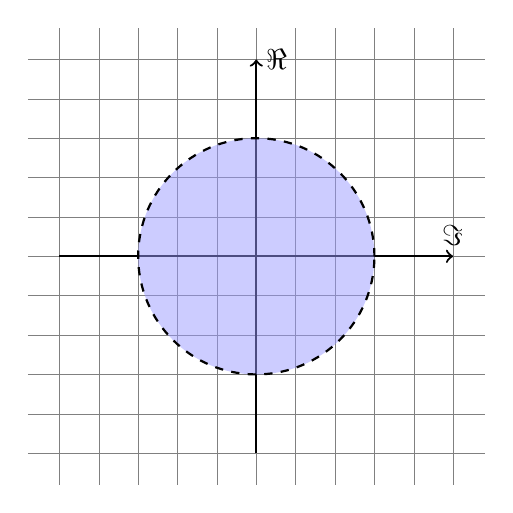
\begin{tikzpicture}
		\draw[step=0.5, black!10!white, help lines](-2.9,-2.9) grid (2.9, 2.9);
		\draw[thick, ->] (-2.5,0) -- (2.5,0) node[anchor=south] {$\Im$};
		\draw[thick, ->] (0,-2.5) -- (0,2.5) node[anchor=west]{$\Re$};
		\filldraw[blue!40!white, thick, dashed, draw=black, fill opacity=0.5] (0,0) circle (1.5cm);
	\end{tikzpicture}
	\caption{The planar set representing $ |z| \le 3 $}
\end{figure}



\begin{figure}[h!]
	\centering
	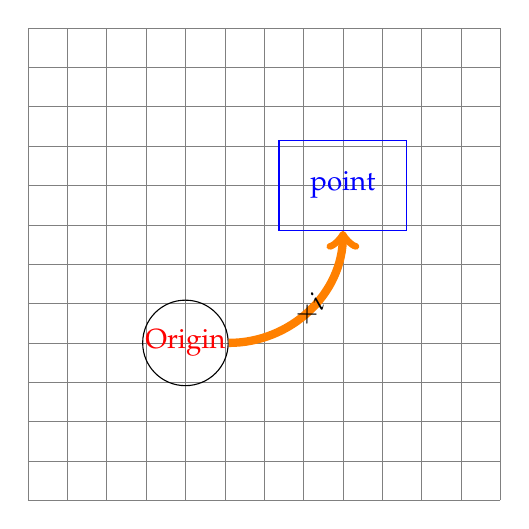
\begin{tikzpicture}[inner sep=4mm]
		\draw [step=0.5, gray, very thin] (-2,-2) grid (4,4);
		\coordinate (O) at (0,0);
		\coordinate (A) at (2,2);
		\node[red, circle, draw=black,inner sep=0.1] (P1) at (O) {Origin};
		\node[blue, rectangle, draw] (P2) at (A) {point};
%		\path (O) node[circle,draw](O) {Origin} (A) node[circle,draw](A) {h};
		\draw[->,orange,line width=3] (P1) to[out=0, in=-90] node[pos=0.5,sloped,black]{$\times i$} (P2);

	\end{tikzpicture}
	\caption{Practicing with nodes}
\end{figure}


\begin{figure}[h!]
	\centering
	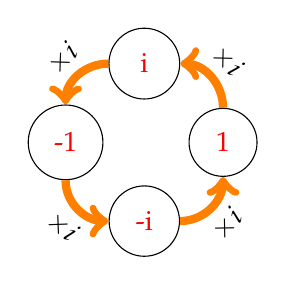
\begin{tikzpicture}[inner sep=4mm]
%		\draw [step=0.5, gray!50!white, line width=0.1] (-2,-2) grid (2,2);
		\node[red, circle, draw=black,inner sep=0.2cm] (1) at (1,0) {1};
		\node[red, circle, draw=black,inner sep=0.23cm] (i) at (0,1) {i};
		\node[red, circle, draw=black,inner sep=0.2cm] (-1) at (-1,0) {-1};
		\node[red, circle, draw=black,inner sep=0.2cm] (-i) at (0,-1) {-i};
		\draw[->, orange, line width=3] (1) to[out=90, in=0] node[sloped, black, anchor=south,inner sep=1mm] {$\times i$} (i);
		\draw[->, orange, line width=3] (i) to[out=-180, in=90] node[sloped, black, anchor=south,inner sep=1mm] {$\times i$} (-1);
		\draw[->, orange, line width=3] (-1) to[out=-90, in=180] node[sloped, black, anchor=north,inner sep=1mm] {$\times i$} (-i);
		\draw[->, orange, line width=3] (-i) to[out=0, in=-90] node[sloped, black, anchor=north,inner sep=1mm] {$\times i$} (1);
	\end{tikzpicture}
	\caption{Practicing with nodes}
\end{figure}




\begin{figure}
	\centering
	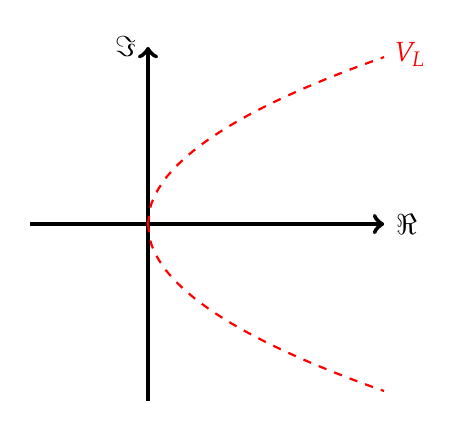
\begin{tikzpicture}[scale=1.5]
		\draw [->, ultra thick] (-1,0) -- (2,0) node [right] {$\Re$};
		\draw [->, ultra thick] (0,-1.5) -- (0,1.5) node [left] {$\Im$};
		\draw[thick,samples=100,smooth,variable=\x,domain=0:2,red, dashed]
		plot(\x,{(\x)^0.5}) node[above=1,right] {$V_L$}
		plot(\x,{-(\x)^0.5});
	\end{tikzpicture}
	\caption{Plotting the functions}
\end{figure}


\begin{figure}
	\centering
	\begin{tikzpicture}[scale=1.5]
		\draw[->, ultra thick] (-1,0) -- (2,0) node [right] {$\Re$};
		\draw[->, ultra thick] (0,-1.5) -- (0,1.5) node [left] {$\Im$};
		\draw[thick, dashed] (0.5,1.5) -- (0.5,-1.5);
		\tick{0.5,0}{90} node[scale=1,below,fill=gray!15] {$\frac{1}{2}$};
	\end{tikzpicture}
	\caption {Sample plot in $\mathbb{C}$}
\end{figure}


\begin{figure}[h!]
	\centering
	\begin{tikzpicture}[scale=2]
		\def\xmax{2.0}
		\def\ymax{1.6}
		\def\R{1.9}
		\def\ang{35}
		\coordinate (O) at (0,0);
		\coordinate (R) at (\ang:\R);
		\coordinate (-R) at (-\ang:\R);
		\coordinate (X) at ({\R*cos(\ang)},0);
		\coordinate (Y) at (0,{\R*sin(\ang)});
		\coordinate (-Y) at (0,{-\R*sin(\ang)});
		\node[fill=mydarkblue,circle,inner sep=0.8] (point) at (R) {};
		
		\node[mydarkblue,above right=-2] at (R) {$z=x+iy=re^{i\phi}$};
		
		\draw[dashed,mydarkblue] (Y) -- (point) -- ++ (0,{0.1-\R*sin(\ang)});
		
		\draw[->,ultra thick] (-0.2*\xmax,0) -- (\xmax+0.05,0) node[right] {Re};
		\draw[->,ultra thick] (0,-\ymax*0.2) -- (0,\ymax+0.05) node[left] {Im};
		\draw[vector] (O) -- (point) node[pos=0.55,above left=-2] {$r$};
		
		\draw pic[->,"$\theta$",mydarkblue,draw=mydarkblue,angle radius=23,angle eccentricity=1.24]
		{angle = X--O--R};
		
		%\tick{X}{90} node[scale=0.9,left=6,below right=-2] {$x = r\cos\theta$};
		\tick{X}{90} node[mydarkblue,scale=1,below=-1] {$x$};
		\tick{Y}{ 0} node[mydarkblue,scale=1,left] {$y$}; %r\sin\theta = 
		
	\end{tikzpicture}
	\caption{A summary of the polar and Cartesian representation of the complex numbers.}
\end{figure}












\end{document}